\section{APIs \& Shading Languages}

\subsection{Graphics APIs}
\begin{frame}{Graphics APIs Overview}
  \begin{columns}
    \begin{column}{0.7\textwidth}
      \begin{conceptbox}{What is a Graphics API?}
        An \textbf{Application Programming Interface} that provides:
        \begin{itemize}
          \item Commands to control the GPU
          \item Abstraction over hardware differences
          \item Standard interface for graphics operations
        \end{itemize}
      \end{conceptbox}
    \end{column}
    \begin{column}{0.3\textwidth}
      \begin{center}
        \begin{tikzpicture}[scale=0.8]
          \node[rectangle, draw, fill=PrimaryColor!20, minimum width=2.5cm, minimum height=0.8cm] (app) at (0,4.5) {Application};
          \node[rectangle, draw, fill=SecondaryColor!20, minimum width=2.5cm, minimum height=0.8cm] (api) at (0,3) {Graphics API};
          \node[rectangle, draw, fill=ObjectColor!20, minimum width=2.5cm, minimum height=0.8cm] (driver) at (0,1.5) {Driver};
          \node[rectangle, draw, fill=LightGray, minimum width=2.5cm, minimum height=0.8cm] (gpu) at (0,0) {GPU Hardware};

          \draw[->, thick] (app) -- (api);
          \draw[->, thick] (api) -- (driver);
          \draw[->, thick] (driver) -- (gpu);
        \end{tikzpicture}
      \end{center}
    \end{column}
  \end{columns}
\end{frame}

\begin{frame}{Major Graphics APIs}
  \small
  \begin{columns}
    \begin{column}{0.7\textwidth}
      \begin{conceptbox}{OpenGL}
        \textbf{Open Graphics Library}\\
        Perhaps the most widely used and most beginner-friendly graphics API.
        OpenGL was designed to be a cross-platform standard for rendering 2D and 3D graphics.
        \begin{itemize}
          \item Stable APIs
          \item High-level abstraction
          \item \faIcon{linux}, \faIcon{android}, \faIcon{windows} Support
          \item Two modes -
            \begin{itemize}
              \item \textbf{Immediate Mode} - Deprecated, fixed function (Used by iGraphics)
              \item \textbf{Retained Mode} - Modern OpenGL, uses shaders
            \end{itemize}
        \end{itemize}
      \end{conceptbox}
    \end{column}
    \begin{column}{0.3\textwidth}
      \begin{center}
        
\includegraphics[width=0.8\textwidth]{images/Opengl-logo.png}
      \end{center}
    \end{column}
  \end{columns}
\end{frame}

\begin{frame}{Major Graphics APIs}
  \small
  \begin{columns}
    \begin{column}{0.7\textwidth}
      \begin{conceptbox}{Vulkan}
        \textbf{Low-overhead, Cross-platform Graphics API} \\
        Developed by the Khronos Group as a modern successor to OpenGL.
        Designed for high-performance, multi-threaded rendering.
        \begin{itemize}
          \item Low-level control over GPU
          \item Better CPU-GPU parallelism
          \item Explicit memory and resource management
          \item \faIcon{linux}, \faIcon{android}, \faIcon{windows} Support
          \item \faIcon{apple} Support via MoltenVK
        \end{itemize}
      \end{conceptbox}
    \end{column}
    \begin{column}{0.3\textwidth}
      \hspace*{-0.7cm}
      
\includegraphics[width=1.3\textwidth]{images/Vulkan_logo..png}
    \end{column}
  \end{columns}
\end{frame}

\begin{frame}{Major Graphics APIs}
  \small
  \begin{columns}
    \begin{column}{0.7\textwidth}
      \begin{conceptbox}{DirectX (Direct3D)}
        \textbf{Microsoft's Graphics API for Windows and Xbox} \\
        A powerful API suite used primarily for game development on Windows platforms.
        \begin{itemize}
          \item Direct3D for 3D rendering
          \item Deep integration with Windows OS and drivers
          \item High performance with hardware vendor optimizations
          \item \faIcon{windows}, \faIcon{xbox} Support only
        \end{itemize}
      \end{conceptbox}
    \end{column}
    \begin{column}{0.3\textwidth}
      \begin{center}
        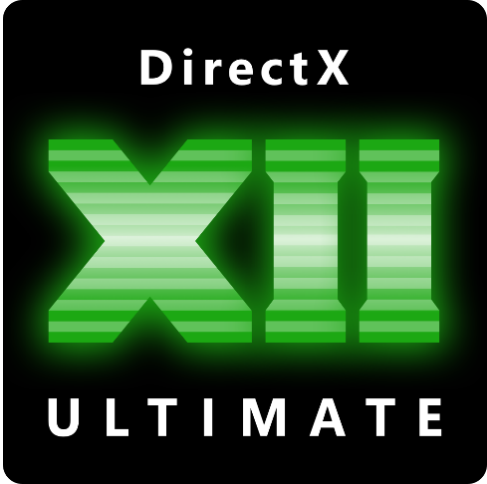
\includegraphics[width=0.7\textwidth]{images/DirectX_12_Ultimate.png}
      \end{center}
    \end{column}
  \end{columns}
\end{frame}

\begin{frame}{Major Graphics APIs}
  \small
  \begin{columns}
    \begin{column}{0.7\textwidth}
      \begin{conceptbox}{Metal}
        \textbf{Apple's Low-level Graphics API} \\
        Designed to maximize performance on Apple devices, replacing OpenGL on Apple platforms.
        \begin{itemize}
          \item Low-overhead, low-level access
          \item Unified graphics and compute
          \item Tight integration with Apple hardware
          \item \faIcon{apple} Support only (macOS, iOS, iPadOS)
        \end{itemize}
      \end{conceptbox}
    \end{column}
    \begin{column}{0.3\textwidth}
      \begin{center}
        
\includegraphics[width=0.8\textwidth]{images/Metal_4.png}
      \end{center}
    \end{column}
  \end{columns}
\end{frame}

\subsection{Shading Languages}
\begin{frame}{Shading Languages}
  \begin{columns}
    \begin{column}{0.6\textwidth}
      \begin{conceptbox}{Purpose}
        Shading languages allow programmers to write code that runs on the GPU for:
        \begin{itemize}
          \item \textbf{Vertex processing} (transformations)
          \item \textbf{Fragment processing} (lighting, texturing, effects)
          \item \textbf{Compute operations} (general-purpose GPU computing)
        \end{itemize}
      \end{conceptbox}
    \end{column}
    \begin{column}{0.4\textwidth}
      \small
      \textbf{Major Shading Languages:}
      \begin{itemize}
        \item \textcolor{PrimaryColor}{\textbf{GLSL}} (OpenGL)
        \item \textcolor{SecondaryColor}{\textbf{HLSL}} (DirectX)
        \item \textcolor{ObjectColor}{\textbf{MSL}} (Metal)
        \item \textcolor{AccentColor}{\textbf{SPIR-V}} (Vulkan) \\
          {\footnotesize Can be compiled from \\ GLSL or HLSL}
      \end{itemize}
    \end{column}
  \end{columns}
\end{frame}

\subsection{GLSL Overview}
\begin{frame}[fragile]{GLSL: OpenGL Shading Language}
  \begin{columns}
    \begin{column}{0.5\textwidth}
      \small
      \begin{raybox}{GLSL Characteristics}
        \footnotesize
        \begin{itemize}
          \item C-like syntax
          \item Built-in vector/matrix types
          \item Version-specific features
        \end{itemize}
      \end{raybox}

      \begin{mathbox}{Data Types}
        \footnotesize
        \begin{itemize}
          \item \texttt{float, int, bool}
          \item \texttt{vec2, vec3, vec4}
          \item \texttt{mat2, mat3, mat4}
          \item \texttt{sampler2D, samplerCube}
        \end{itemize}
      \end{mathbox}
    \end{column}
    \begin{column}{0.5\textwidth}
      \begin{minted}[fontsize=\scriptsize, bgcolor=LightGray!20]{glsl}
#version 330 core
// Vertex shader inputs
layout (location = 0) in vec3 aPos;
layout (location = 1) in vec3 aNormal;
layout (location = 2) in vec2 aTexCoord;
// Outputs to fragment shader
out vec3 FragPos;
out vec3 Normal;
out vec2 TexCoord;
// Uniform variables
uniform mat4 model;
uniform mat4 view;
uniform mat4 projection;

void main() {
    FragPos = vec3(model * vec4(aPos, 1.0));
    Normal = mat3(transpose(inverse(model)))
              * aNormal;
    TexCoord = aTexCoord;

    gl_Position = projection
                  * view
                  * vec4(FragPos, 1.0);
}
      \end{minted}
    \end{column}
  \end{columns}
\end{frame}

\begin{frame}[fragile]{GLSL Qualifiers}
  \begin{columns}
    \begin{column}{0.5\textwidth}
      \begin{conceptbox}{Storage Qualifiers}
        \footnotesize
        \begin{itemize}
          \item \texttt{\textcolor{PrimaryColor}{in}} - Input from previous stage
          \item \texttt{\textcolor{SecondaryColor}{out}} - Output to next stage
          \item \texttt{\textcolor{ObjectColor}{uniform}} - Buffer from CPU
        \end{itemize}
      \end{conceptbox}

      \begin{mathbox}{Layout Qualifiers}
        \footnotesize
        Used to explicitly assign indices or binding points to resources.
        \begin{itemize}
          \item \texttt{location} - Attribute/output index
          \item \texttt{binding} - Texture/uniform buffer slot
        \end{itemize}
      \end{mathbox}
    \end{column}
    \begin{column}{0.5\textwidth}
      \begin{minted}[fontsize=\scriptsize, bgcolor=LightGray!20]{glsl}
#version 330 core
// Fragment shader
in vec3 FragPos;
in vec3 Normal;
in vec2 TexCoord;
out vec4 FragColor;
uniform vec3 lightPos;
uniform vec3 viewPos;
uniform sampler2D texture_diffuse1;
void main() {
    vec3 color = texture(texture_diffuse1,
                          TexCoord).rgb;
    // Ambient
    vec3 ambient = 0.1 * color;
    // Diffuse
    vec3 norm = normalize(Normal);
    vec3 lightDir = normalize(
                      lightPos - FragPos);
    float diff = max(dot(norm, lightDir),
                      0.0);
    vec3 diffuse = diff * color;
    // Result
    vec3 result = ambient + diffuse;
    FragColor = vec4(result, 1.0);
}
      \end{minted}
    \end{column}
  \end{columns}
\end{frame}
